\chapter{Beyond Basic Socket Programming}
\label{chap:advanced}

Our client and server examples
demonstrate the basic model for socket programming.  The next step is
to integrate these ideas into various programming models such as
multitasking, signalling, and broadcasting.  We demonstrate these
principles in the context of standard UNIX programming; however, most
modern operating systems support similar features (e.g., processes
and threads).

\section{Socket Options}
\label{sect:socketoptions}

\noindent The TCP/IP protocol developers spent a good deal of time
thinking about the default behaviors that would satisfy most
applications.  (If you doubt this, 
read RFCs 1122 and 1123, which describe in excruciating detail
the recommended behaviors---based on years of experience---for 
implementations of the TCP/IP protocols.)
For most applications, the designers did a good job; however, it is
seldom the case that ``one-size-fits-all'' really fits all.  For
example, each socket has an associated receive buffer.
How big should it be?  Each implementation has
a default size; however, this value may not always be appropriate for
your application (see also \Sect{sect:sendrec}).
This particular aspect of a socket's behavior, along with many others,
is associated with a \defn{socket option}: You can
change the receive
buffer size of a socket by modifying the value of the associated
socket option.  The functions \fcnrefsys{getsockopt()} and
\fcnrefsys{setsockopt()} allow
socket option values to be queried and set, respectively.

\begin{inlinefcn}
\type{int} \fcnrefsys{getsockopt}(\type{int} \param{socket}, \type{int} \param{level}, \type{int} \param{optName}, \type{void *}\param{optVal}, \type{unsigned int *}\param{optLen}) \\
\type{int} \fcnrefsys{setsockopt}(\type{int} \param{socket}, \type{int} \param{level}, \type{int} \param{optName}, \type{const void *}\param{optVal}, \type{unsigned int} \param{optLen})
\end{inlinefcn}
For both functions, \param{socket} must be a socket descriptor 
allocated by \fcnrefsys{socket()}.  
The available socket options are divided
into levels that correspond to the layers of the
protocol stack; the second parameter indicates the level of the option
in question.
Some options are protocol independent and are thus
handled by the socket layer itself  (\const{sol\_socket}),
some are specific to the transport protocol
(\const{ipproto\_tcp}),
and some are handled by the internetwork  protocol
(\const{ipproto\_ip}).
The option itself is specified by the integer \param{optName}, which
is always specified using a system-defined constant.
The parameter \param{optVal}
is a pointer to a buffer.  For \fcnrefsys{getsockopt()},
the option's current value will placed in that buffer by the
implementation, whereas
for \fcnrefsys{setsockopt()},
the socket option in the implementation will be
set to the value in the buffer.
In both calls, \param{optLen} specifies the length of the
buffer, which must be correct
for the particular option in question.
Note that in \fcnrefsys{getsockopt()}, \param{optLen} is an
in-out parameter,
initially pointing to an integer containing
the size of the buffer; on return the pointed-to integer contains
the size of the option value.
The following code segment demonstrates how to fetch and then double
the configured size (in bytes) of the socket's receive buffer:

\label{code:socketoption}
\begin{inlinecode}
int rcvBufferSize;
// Retrieve and print the default buffer size
int sockOptSize = sizeof(rcvBufferSize);
if (getsockopt(sock, SOL_SOCKET, SO_RCVBUF, &rcvBufferSize, &sockOptSize) < 0)
    DieWithSystemMessage("getsockopt() failed");
printf("Initial Receive Buffer Size: %d\\n", rcvBufferSize);

// Double the buffer size
rcvBufferSize *= 2;
if (setsockopt(sock, SOL_SOCKET, SO_RCVBUF, &rcvBufferSize, sizeof(rcvBufferSize)) < 0)
    DieWithSystemMessage("setsockopt() failed");
\end{inlinecode}

Note that value passed to \fcn{setsockopt()} is \emph{not\/}
guaranteed to be the new size of the socket buffer, even if the call
apparently succeeds.  Rather, it is best thought of
as a ``hint'' to the system about the value desired by the user; the
system, after all, has to manage resources for \emph{all\/} users, and
may consider other factors in adjusting buffer size.

Table~\ref{fig:sockopts} shows some commonly used options at each
level, including a description and the data type of the
buffer pointed to by \param{optVal}.  

%
\begin{table}[htbp]
%\caption{\label{fig:sockopts}Socket Options}
%
% option | Type | Values | Description
\noindent \begin{tabular}{l||c|c|p{2.4in}}
\multicolumn{4}{l}{\textbf{SOL\_SOCKET}} \\
optname & Type & Values & Description \\ \hline \hline
SO\_BROADCAST & \type{int} & 0,1 & Broadcast allowed \\ \hline
SO\_KEEPALIVE & \type{int} & 0,1 & Keepalive
messages enabled (if implemented by protocol) \\ \hline
SO\_LINGER & \type{linger$\lbrace\rbrace$} & time &
Time to delay \fcnrefsys{close} return waiting for confirmation
(see \Sect{sect:lifecycle})\\ \hline
SO\_RCVBUF & \type{int} & bytes & Bytes in the socket receive buffer (see
code on page~\pageref{code:socketoption} and \Sect{sect:sendrec}) \\ \hline
SO\_RCVLOWAT & \type{int} & bytes & Minimum number of
available bytes that will cause \fcnrefsys{recv} to return \\ \hline
SO\_REUSEADDR & \type{int} & 0,1 & Binding allowed
(under certain conditions) to an address or port already in
use (see \Sect{sect:lifecycle})  \\ \hline
SO\_SNDLOWAT & \type{int} & bytes & Minimum bytes
to send \\ \hline % ?????XXXXX
SO\_SNDBUF & \type{int} & bytes & Bytes
in the socket send buffer (see  \Sect{sect:sendrec})\\ \hline
%SO\_TYPE & \type{int} & socket type & Type of the socket
%(SOCK\_STREAM or SOCK\_DGRAM) - Get only. \\ \hline
%
\multicolumn{4}{l}{\raisebox{-1em}{\textbf{IPPROTO\_TCP}}} \\
% option | Type | Values | Description
optname & type & Values & Description \\ \hline \hline
TCP\_MAX & \type{int} & seconds &
Seconds between keepalive messages. \\ \hline
%TCP\_MAXRT & \type{int} & -1, 255&
%Maximum TCP segment size. \\ \hline
TCP\_NODELAY & \type{int} & 0, 1&
Disallow delay from Nagle's algorithm for data merging \\ \hline
%
\multicolumn{4}{l}{\raisebox{-1em}{\textbf{IPPROTO\_IP}}}\\
% option | Type | Values | Description
optname & type & Values & Description \\ \hline \hline
IP\_TTL & \type{int} & 0 - 255 &
Time-to-live for unicast IP packets. \\ \hline
IP\_MULTICAST\_TTL & \type{unsigned char} & 0 - 255 &
Time-to-live for multicast IP packets
(see \file{MulticastSender.c} on pg.~\pageref{code/MulticastSender.c})\\ \hline
IP\_MULTICAST\_LOOP & \type{int} & 0,1 &
Enables multicast socket to receive packets it sent \\ \hline
IP\_ADD\_MEMBERSHIP & \type{ip\_mreq$\lbrace\rbrace$} & group address &
Enables reception of packets addressed to the specified multicast group
(see \file{MulticastReceiver.c} on pg.~\pageref{code/MulticastReceiver.c}) -- Set only \\ \hline
IP\_DROP\_MEMBERSHIP & \type{ip\_mreq$\lbrace\rbrace$} & group address &
Disables reception of packets addressed to the specified multicast
group -- Set only \\ \hline
%
\multicolumn{4}{l}{\raisebox{-1em}{\textbf{IPPROTO\_IPV6}}}\\
% option | Type | Values | Description
optname & type & Values & Description \\ \hline \hline
IPV6\_V6ONLY & \type{int} & 0,1 &
Restrict IPv6 sockets to only IPv6 communication. \\ \hline
IPV6\_UNICAST\_HOPS & \type{int} & -1 - 255 &
Time-to-live for unicast IP packets. \\ \hline
IPV6\_MULTICAST\_HOPS & \type{int} & -1 - 255 &
Time-to-live for multicast IP packets
(see \file{MulticastSender.c} on pg.~\pageref{code/MulticastSender.c})\\ \hline
IPV6\_MULTICAST\_LOOP & \type{u\_int} & 0,1 &
Enables multicast socket to receive packets it sent \\ \hline
IPV6\_JOIN\_GROUP & \type{ipv6\_mreq$\lbrace\rbrace$} & group address &
Enables reception of packets addressed to the specified multicast group
(see \file{MulticastReceiver.c} on pg.~\pageref{code/MulticastReceiver.c}) -- Set only \\ \hline
IPV6\_LEAVE\_GROUP & \type{ipv6\_mreq$\lbrace\rbrace$} & group address &
Disables reception of packets addressed to the specified multicast
group -- Set only \\ \hline
\end{tabular}
\caption{\label{fig:sockopts}Socket Options}
\end{table}

\section{Signals}
\label{sect:signals}%

\noindent Signals provide a mechanism for notifying programs that certain events
have occurred---for example,
the user typed the ``interrupt'' character, or a timer expired.
Some of the events (and therefore the notification)
may occur \emph{asynchronously}, 
which means that the notification is delivered to the
program regardless of which statement it is executing.
When a signal is delivered to a running program,
one of four things happens:

\begin{enumerate}
\item The signal is ignored. The process is never aware that the signal was
delivered.
\item The program is forcibly terminated by the operating system.
\item Program execution is interrupted and
a \emph{signal-handling routine}, specified by (and part of) the
program, is executed. This execution happens in a different thread
of control from the main thread(s) of  the program so that the
program is not necessarily immediately aware of it.
\item The signal is \emph{blocked}, that is, prevented from having any effect
until the program takes action to allow its delivery.
Each process has a \emph{mask}, indicating which signals are
currently blocked in that process. (Actually, each thread in a
program can have its own signal mask.)
\end{enumerate}

UNIX has dozens of different signals, each indicating the occurrence
of a different type of event.
Each signal has a system-defined \emph{default behavior}, which is one of
the first two possibilities listed above.  For example, termination is the
default behavior for \const{sigint},
which is delivered when the interrupt  character  (usually Control-C)
is received via the controlling terminal for that process.

Signals are a complicated animal, and a full treatment is beyond the
scope of this book.  However, some signals are frequently encountered
in the context of socket programming.  Moreover,
\callout{any program that sends
on a TCP socket must explicitly deal with 
% XXXX inside \callout the small caps thing doesn't work...
\const{SIGPIPE} in order to be robust.}
Therefore, we present the basics of dealing with signals,
focusing on these five:
%
\begin{center}
\begin{tabular}{|l|l|l|} \hline
Type & Triggering Event & Default \\ \hline \hline
\constsys{sigalrm} & Expiration of an alarm timer & termination \\ \hline
\constsys{sigchld} & Child process exit & ignore \\ \hline
\constsys{sigint} & Interrupt char (Control-C) input & termination \\ \hline
\constsys{sigio} & Socket ready for I/O & ignore \\ \hline
\constsys{sigpipe} & Attempt to write to a closed socket & termination \\ \hline
\end{tabular}
\end{center}
%
An application program can change the default behavior\footnote{For some
signals, the default behavior cannot be changed nor can the signal
be blocked; however, this is not true for any of the five we consider.}
for a particular signal using \fcnrefsys{sigaction()}:

\begin{inlinefcn}
\type{int} \fcnrefsys{sigaction} (\type{int} \param{whichSignal},
 \type{const struct sigaction *}\param{newAction},\\
\hspace*{1in}\type{struct sigaction *}\param{oldAction})
\end{inlinefcn}

\noindent \fcnrefsys{sigaction()} returns $0$ on success and
$-1$ on failure; details of its semantics, however, are a
bit more involved.

Each signal is identified by an integer constant;
\param{whichSignal} specifies the signal for which the behavior is
being changed.
The \param{newAction} parameter points to a
\type{sigaction} structure that defines the
new behavior for the given signal type; if the pointer
\param{oldAction} is non-null, a \type{sigaction}
structure 
describing the previous behavior for the given signal is copied into it, as
shown here:

\label{page:sigactionstruct}
\begin{inlinecode}
struct sigaction {
    void (*sa_handler)(int);  // Signal handler
    sigset_t sa_mask;         // Signals to be blocked during handler execution
    int sa_flags;             // Flags to modify default behavior
};
\end{inlinecode}

The field \structmem{sa\_handler} (of type ``pointer to function of
one integer parameter that returns void'') controls
which of the first three possibilities occurs when
a signal is delivered (i.e., when it is not masked).
If its value is the special constant \const{sig\_ign},
the signal will be ignored.  If its value is \const{sig\_dfl}, the
default behavior for that signal will be used.
If its value is the address of a function (which
is guaranteed to be different from the two constants),
that function will be invoked with a parameter indicating the signal
that was delivered.  (If the same
handler function is used for multiple signals, the parameter
can be used to determine which one  caused the invocation.)

Signals can be ``nested'' in the following sense:
While one signal is being handled, another is delivered.
As you can imagine, this can get rather complicated.
Fortunately, the \fcnrefsys{sigaction()} mechanism allows
some signals to be temporarily blocked (in addition to those that are
already blocked by the process's signal mask) while the specified signal is
handled.
The field \structmem{sa\_mask} specifies the
signals to be blocked while 
handling \param{whichSignal}; it is only meaningful when
\structmem{sa\_handler} is not \const{sig\_ign} or
\const{sig\_dfl}.  By default \param{whichSignal} is always
blocked regardless of whether it is reflected in
\structmem{sa\_mask}. (On some systems, setting 
the flag \const{sa\_nodefer} in \structmem{sa\_flags}
allows the specified signal to be delivered while it is being handled.)
The \structmem{sa\_flags} field controls some further details of the
way \param{whichSignal} is handled; these details are beyond the scope of this
discussion.

\structmem{sa\_mask} is implemented as a set of boolean flags, one for
each type of signal.  This set of flags can be manipulated with the following
four functions:

\begin{inlinefcn}
\type{int} \fcnrefsys{sigemptyset}(\type{sigset\_t *}\param{set})\\
\type{int} \fcnrefsys{sigfillset}(\type{sigset\_t *}\param{set})\\
\type{int} \fcnrefsys{sigaddset}(\type{sigset\_t *}\param{set}, \type{int} \param{whichSignal})\\
\type{int} \fcnrefsys{sigdelset}(\type{sigset\_t *}\param{set}, \type{int} \param{whichSignal})
\end{inlinefcn}

\noindent \fcnrefsys{sigfillset()} and
\fcnrefsys{sigemptyset()} set and
unset all of the flags in the given set. 
\fcnrefsys{sigaddset()} and
\fcnrefsys{sigdelset()} set and unset individual flags,
specified by the
signal number, in the given set.  All four functions return $0$ for
success and $-1$ for failure.

\file{SigAction.c} shows a simple \fcnrefsys{sigaction()}
example to
provide a handler for SIGINT by setting up a signal handler and then
entering an infinite loop.  When the program receives an interrupt
signal, the handler function, a pointer to which is supplied to
\fcnrefsys{sigaction()},
executes and exits the program.

\jcode{SigAction.c}{code/SigAction.c}{1}{1}

\begin{topcode}
\tlcitem{Signal handler function prototype}{5}

\tlcitems{Set up signal handler}{9--21}

\begin{bottomcode}
\blcitem{Assign function to handle signal}{12}

\blcitems{Fill signal mask}{14--15}

\blcitems{Set signal handler for SIGINT}{20--21}

\end{bottomcode}

\tlcitems{Loop forever until SIGINT}{23--24}

\fcnrefsys{pause()} suspends the process until a signal is received.

\tlcitems{Function to handle signal}{29--33}

\fcnrefsys{InterruptSignalHandler()} prints a message and exits the program.

\end{topcode}

So what happens when a signal that would otherwise be delivered is
blocked, say, because another signal is being handled?
Delivery is postponed until the handler completes. Such a signal is said to
be \emph{pending}.
\callout{It is important to realize that
signals are \emph{not} queued---a signal is either
pending or it is not.}  If the same signal is delivered more than once
while it is being handled, the handler is only executed
once more after it completes the original execution.
Consider the case where three SIGINT signals arrive while
the signal handler for SIGINT is already executing.  The first of the
three SIGINT signals is blocked; however, the subsequent two signals
are lost.  When the SIGINT signal handler function completes, the
system executes the handler only \emph{once} again.  We must be
prepared to handle this behavior in our applications.
To see this in action, modify 
\fcnrefsys{InterruptSignalHandler()} in \file{SigAction.c} as follows:

\begin{inlinecode}
void InterruptSignalHandler(int ignored) {
      printf("Interrupt Received.\n");
      sleep(3);
}
\end{inlinecode}

\noindent The signal handler for SIGINT sleeps for three seconds and
returns, instead of exiting.  Now when you execute the program, hit the
interrupt key (Control-C) several times in succession.  If you
hit the interrupt key more than two times in a row,
you still only see two ``Interrupt Received'' messages.
The first interrupt signal invokes
\fcnref{InterruptSignalHandler()}, which sleeps
for three seconds.  The
second interrupt is blocked because SIGINT is already being handled.
The third and fourth interrupts are lost.  Be warned that you
will no longer be able to stop your program with a keyboard interrupt.  You
will need to explicitly send another signal (such as
\const{SIGTERM}) to the process using the \type{kill}
command.

One of the most important aspect of signals relates to the
sockets interface.  If a signal is delivered while the program is
blocked in a socket call (such as a \fcnrefsys{recv()} or
\fcnrefsys{connect()}), and a handler for that signal
has been specified, as soon as
the handler completes, the socket call will return $-1$ with
\var{errno}\ set to \const{EINTR}.
Thus, \callout{your programs that catch and handle signals need to
be prepared for these erroneous returns from system calls that can block.}

Later in this chapter we encounter the first four signals mentioned
above.  Here we briefly describe the semantics of
\const{SIGPIPE}.
Consider the following scenario: A server (or client) has a connected
TCP socket, and the other end abruptly and
unexpectedly closes the connection, say,
because the  program crashed.   How does the server find out that the
connection is broken?  The answer is that it doesn't, until it tries
to send on the socket.  At that point, \const{SIGPIPE} is
delivered.  Thus, \const{SIGPIPE} is delivered
\emph{synchronously} and not asynchronously.
(Why not just return $-1$ from \fcn{send()}?  See
exercise~\ref{ex:sigpipe} at the end of the chapter.)

This fact is especially significant for servers, because the default behavior
for \const{SIGPIPE} is to terminate the program.  Thus,
servers that don't change this behavior can be terminated by misbehaving
clients.  Servers should always handle \const{SIGPIPE} so
that they can detect the client's disappearance and reclaim any resources that
were in use to service~it.

\section{Nonblocking I/O}
\label{sect:nbio}%

\noindent The default behavior of a socket call is to block until the requested
action is completed.  For example, the \fcnrefsys{recv()} function in
\file{TCPEchoClient.c} (page~\pageref{code/TCPEchoClient.c}) does not
return until at least one message from the echo server is received.  Of
course, a process with a blocked function is suspended by the operating
system.

A socket call may block for several reasons.  Data reception functions
(\fcnrefsys{recv()} and \fcnrefsys{recvfrom()}) block
if data
is not available.  A \fcnrefsys{send()} on a TCP socket may block
if there is not sufficient space to buffer the transmitted data
(see Section~\ref{sect:sendrec}).
Connection-related functions for TCP sockets
block until a connection has been established.
For example, \fcnrefsys{accept()}
in \file{TCPEchoServer.c} (page~\pageref{code/TCPEchoServer.c})
blocks until a client establishes a connection with
\fcnrefsys{connect()}.  Long round-trip times, high
error rate connections, or a slow (or deceased) server may cause a call to
\fcnrefsys{connect()}  to block for a significant amount of time.
In all of these cases, the
function returns only after the request has been satisfied.

What about a program that has other tasks to perform while waiting for
call completion?  (For example, one that
needs to update the ``busy'' cursor or respond to user
requests.)  These programs may have no time to wait on a blocked
system call.  What about lost UDP datagrams?  In
\file{UDPEchoClient.c} (page~\pageref{code/UDPEchoClient.c}), the client sends
a datagram to the server
and then waits to receive a response.
\callout{If either the datagram sent from the
client or the echoed datagram from the server is lost, our echo client
blocks indefinitely.}
In this case, we need
\fcnrefsys{recvfrom()} to
unblock after some amount of time to allow the client to handle the
datagram loss.
Fortunately, several mechanisms are available for  controlling
unwanted blocking behaviors.  We deal
with three here:  nonblocking sockets,
asynchronous I/O, and timeouts.

\subsection{Nonblocking Sockets}

\noindent One obvious solution to the problem of undesirable blocking
is to change the behavior of the socket so that \emph{all\/}
calls are \defn{nonblocking}.  For such a socket, 
if a requested operation can be completed immediately, the call's
return value indicates success; otherwise it indicates failure
(usually $-1$).  In either case the call does not
block indefinitely.  In the case of failure, we need the
ability to distinguish between failure due to blocking and other types
of failures.  If the failure occurred because the call would have 
blocked, the system sets \var{errno}\ to
\const{ewouldblock},\footnote{Some sockets implementations
return
\const{eagain}. On many systems,
\const{eagain} and
\const{ewouldblock} are the same error number.} except for
\fcnrefsys{connect()}, which returns an \var{errno}\ of
\const{einprogress}.

We can change the default blocking behavior with a call to
\fcnrefsys{fcntl()} (``file control'').

\begin{inlinefcn}
\type{int} \fcnrefsys{fcntl}(\type{int} \param{socket}, \type{int} \param{command}, \type{long} \param{argument})
\end{inlinefcn}

\noindent As the name suggests, this call can be used with any kind of file:
\param{socket} must be a valid file (or socket) descriptor.
The operation to be performed is given by \param{command}, which is
\emph{always\/} a system-defined constant.
The behavior we want to modify is controlled by
flags (\emph{not\/} the same as socket options) associated with the
descriptor, which we can get and set with
the \const{f\_getfl} and \const{f\_setfl}
commands.  When setting
the socket flags, we must specify the new flags in \param{argument}.
The flag that controls nonblocking behavior is
\const{o\_nonblock}.
When getting the socket flags, \param{argument} is 0.  We demonstrate
the use of a nonblocking socket in the next section,
where we describe asynchronous I/O in
\file{UDPEchoServer-SIGIO.c} (page~\pageref{code/UDPEchoServer-SIGIO.c}).

There are a few exceptions to this model of nonblocking
sockets.  For UDP sockets, there are no send
buffers, so \fcnrefsys{send()} and \fcnrefsys{sendto()}
never return \const{ewouldblock}.  For all but the
\fcnrefsys{connect()} socket
call, the requested operation either completes before returning
or none of the operation is performed.  For
example, \fcnrefsys{recv()} either receives data from the socket or
returns an error.  A nonblocking \fcnrefsys{connect()} is
different.
For UDP, \fcnrefsys{connect()} simply assigns a destination
address for
future data transmissions so it never blocks.  For TCP,
\fcnrefsys{connect()} initiates the TCP connection setup. 
If the connection cannot be completed without blocking,
\fcnrefsys{connect()} returns an error, setting \var{errno} to
\const{einprogress}, indicating that the socket is still
working on
making the TCP connection.   Of course, subsequent data sends and
receives cannot happen until the connection is established.
Determining when the connection is complete is beyond the scope of
this text,\footnote{Well, mostly.
Connection completion can be detected using the
\fcnrefsys{select()} call, described in
Section~\ref{sect:multiplexing}.} so we
recommend not setting the socket to nonblocking until after the call
to \fcnrefsys{connect()}.

For eliminating blocking during individual send and receive operations,
an alternative is available on some platforms.
The \param{flags} parameter of \fcnrefsys{send()}, \fcnrefsys{recv()},
\fcnrefsys{sendto()}, and \fcnrefsys{recvfrom()} allows for modification
of some aspects of the behavior on a particular call.
Some implementations support the
\const{msg\_dontwait} flag, which
causes nonblocking behavior in
any call where it is set in \param{flags}.

\subsection{Asynchronous I/O}

\noindent The difficulty with nonblocking socket calls is that there is no way
of knowing when one would succeed, except by periodically trying it
until it does (a process known as ``polling'').  Why not have the
operating system inform the program when a socket call will be
successful?  That way the program can spend its time doing other work
until notified that the socket is ready for something to happen.  This
is called \defn{asynchronous I/O}, and it works
by having the
\const{sigio} signal delivered to the process when some I/O--related
event occurs on the socket.

Arranging for \const{sigio} involves three steps.  First, we
inform the system of the desired disposition of the signal using
\fcnrefsys{sigaction()}.  Then, we ensure that signals related
to the socket will be delivered to \emph{this} process (because multiple
processes can have access to the same socket, there might be ambiguity about 
which should get it) by making it the owner of the socket, using
\fcnrefsys{fcntl()}.  Finally, we mark the  socket as being primed
for asynchronous I/O by setting a flag (\const{fasync}),
again via \fcnrefsys{fcntl()}.

In our next example, we adapt \file{UDPEchoServer.c}
(page~\pageref{code/UDPEchoServer.c}) to use
asynchronous I/O with nonblocking socket calls.
The modified server is able to perform
other tasks when there are no clients needing
an echo.  After creating and binding the  socket,
instead of calling \fcnrefsys{recvfrom()} and blocking
until a datagram arrives, the asynchronous
echo server establishes a signal handler for \const{SIGIO}
and begins doing
other work.  When a datagram arrives, the \const{SIGIO} signal
is delivered to the
process, triggering execution of the handler function.  The
handler function calls \fcnrefsys{recvfrom()},
echoes back any received datagrams, and then returns, whereupon the
main program continues whatever it was doing.
Our description details only the code that differs
from the original UDP echo server.

\jcode{UDPEchoServer-SIGIO.c}{code/UDPEchoServer-SIGIO.c}{1}{1}

\begin{topcode}

\tlcitems{Additional include files for \fcnrefsys{fcntl()} and signals}{6--9}

\tlcitems{Prototypes for signal and idle time handler}{14--15}

\fcnref{UseIdleTime()} implements the other tasks of the UDP echo server.
\fcnref{SIGIOHandler()} handles \const{sigio} signals.
\callout{Note well: \fcnref{UseIdleTime()} must be prepared for any ``slow''
system calls---such as reading from a terminal device---to
return $-1$ as a
result of the \const{sigio} signal being delivered and handled}
(in which case it should simply verify that \var{errno}\ is
\const{eintr} and resume whatever it was doing).

\tlcitem{Echo socket descriptor}{17}

We give the echo socket descriptor a global scope so that it can be
accessed by the \const{sigio} handler function.

\tlcitems{Set up signal handling}{23, 49--65}

\var{handler} is the \type{sigaction} structure that
describes
our desired signal-handling behavior.  We fill it in, giving the
address of the handling routine and the set of
signals we want blocked.

\begin{bottomcode}

\blcitem{Fill in the pointer to the desired handler}{49}

\blcitems{Specify signals to be blocked during handling}{51--52}

\blcitems{Specify how to handle the sigio signal}{56--57}

\blcitems{Arrange for SIGIO to go to this process}{60--61}

The \const{f\_setown} command identifies the
process to receive \const{sigio} for this socket.


\blcitems{Set flags for nonblocking and asynchronous I/O}{64--65}
Finally, we mark the socket (with the \const{fasync} flag\footnote{The
name
may be different (e.g., \const{o\_async}) on some platforms.})
to indicate that asynchronous I/O is in use,
so \const{sigio} will be delivered on packet arrival.
(Everything up to this point was just saying \emph{how}
to deal with \const{sigio}.)
Because we do not want
\fcnref{SIGIOHandler()} to block in \fcnrefsys{recvfrom()},
we also set the \const{o\_nonblock} flag.
\end{bottomcode}

\tlcitems{Run forever using idle time when available}{69--70}

\tlcitems{Perform nonechoing server tasks}{75--79}

\tlcitems{Handle asynchronous I/O}{81--110}

This code is very similar to the loop in our earlier
\file{UDPEchoServer.c} (page~\pageref{code/UDPEchoServer.c}).  One difference
is that here we loop
until there are no more pending echo requests to satisfy and then
return; this technique enables the main program thread to continue what it was
doing. 

\begin{bottomcode}

\blcitems{Receive echo request}{91--98}

The first call to \fcnrefsys{recvfrom()} receives the datagram
whose arrival
prompted the \const{sigio} signal.  Additional datagrams
may arrive during execution of the handler,
so the do/while loop continues to call \fcnref{recvfrom()}
until no more datagrams remain to be received.
Because \var{sock} is a nonblocking socket,
\fcnrefsys{recvfrom()} then returns $-1$ with \var{errno}\ set to
\const{ewouldblock}, terminating the loop and the handler
function.

\blcitems{Send echo reply}{104--106}

Just as in the original UDP echo server, \fcnrefsys{sendto()}
repeats the message back to the client.

\end{bottomcode}

\end{topcode}

\subsection{Timeouts}
\label{sect:timeouts}%

\noindent In the previous subsection, we relied on the system to notify our
program of the occurrence of an I/O--related event.
Sometimes, however, we may actually need to know that some I/O event
has \emph{not} happened  for a certain time period.
For example, we have mentioned already that UDP messages can be lost;
in case of such a loss, our UDP echo client (or any other
client that uses UDP, for that matter) will never receive a
response to its request.
Of course, the client
cannot tell directly whether a loss has occurred, so it sets
a limit on how long it will wait for a response.
For example, the UDP echo client might assume that if the server has
not responded to its request within two seconds, the server will
never respond.  The client's reaction to this three-second \emph{timeout}
might be to give up or to try again by resending the request.

The standard method of implementing timeouts
is to set an \fcnrefsys{alarm} before calling a
blocking function.

\begin{inlinefcn}
\type{unsigned int} \fcnrefsys{alarm}(\type{unsigned int} \param{secs})
\end{inlinefcn}

\noindent \fcnrefsys{alarm()} starts a timer, which expires after
the specified number of seconds (\param{secs}); \fcnrefsys{alarm()}
returns the number of seconds remaining for any previously scheduled
alarm (or 0 if no alarm was scheduled).
When the timer expires, a \const{SIGALRM} signal is sent
to the process, and the handler function for \const{SIGALRM}, if
any, is executed.

The code we showed earlier in
\file{UDPEchoClient.c} (page~\pageref{code/UDPEchoClient.c}) has a problem if
either the echo request or
response is lost: The client blocks indefinitely on
\fcnrefsys{recvfrom()}, waiting for a datagram that will never
arrive.  Our next example program, \file{UDPEchoClient-Timeout.c}, 
modifies the original UDP echo client
to retransmit the request message if a response from the
echo server is not received within a time limit of two seconds.
To implement this, the new client installs a handler for
\const{SIGALRM}, and just before calling
\fcnrefsys{recvfrom()}, it sets an alarm for two seconds.
At the end of that interval of time,
the \const{SIGALRM} signal is delivered, and the handler
is invoked.
When the handler returns, 
the blocked \fcnrefsys{recvfrom()} returns $-1$ with
\var{errno}\ equal to
\const{EINTR}. The client then resends the echo request to the
server.  This timeout and retransmission of the echo request happens
up to five times before the client gives up and reports failure.  Our
program description only details the code that differs from the original UDP
echo client. 

\jcode{UDPEchoClient-Timeout.c}{code/UDPEchoClient-Timeout.c}{1}{1}

\begin{topcode}

\tlcitems{Additional include files for \var{errno}\ and signals}{6--7}

\tlcitems{Timeout setup}{10--16}

\var{tries} is a global variable so that it can be accessed in the
signal handler.

\tlcitems{Establish signal handler for SIGALRM}{54--60}

This is similar to what  we did for \const{SIGIO} in
\file{UDPEchoServer-SIGIO.c}.

\tlcitem{Set the alarm timer}{76}

When/if the alarm timer expires, the handler \fcnref{CatchAlarm()}
will be invoked.


\tlcitems{Retransmission loop}{77--93}

We have to loop here because the \const{SIGALRM} will cause 
the \fcnref{recvfrom()} to return $-1$.  When that
happens, we decide whether it was  a timeout or not and, if so, retransmit.

\begin{bottomcode}

\blcitems{Attempt reception}{77--78}

\blcitems{Discover the reason for \fcnref{recvfrom()}
failure}{79--93}

If \var{errno}\ equals \constsys{eintr},
\fcnref{recvfrom()} returned
because it was interrupted by the \constsys{sigalrm} while
waiting
for datagram arrival and not because we  got a packet.  In this case
we assume either the echo request or reply is lost.  If we have not
exceeded the maximum number of retransmission attempts, we retransmit
the request to the server; otherwise, we report a failure.  After
retransmission, we reset the alarm timer to wake us again if the
timeout expires.

\end{bottomcode}

\tlcitems{Handle echo response reception}{96--100}

\begin{bottomcode}

\blcitem{Cancel the alarm timer}{96}

\blcitem{Ensure that message is null-terminated}{99}

\fcnrefsys{printf()} will output bytes  until it encounters a null byte,
so we need to make sure one is present (otherwise, our program may crash).

\blcitem{Print the received message}{100}

\end{bottomcode}

\end{topcode}

\section{Multitasking}

\noindent Our TCP echo server handles one client at a time.
If additional clients connect while one is already being
serviced, their connections will be established and they will be able
to send their requests, but the server will not echo back their data
until it has finished with the first client.
This type of socket
application is called an \defn{iterative server}.
\callout{Iterative servers
work best for applications where each client requires a small, bounded
amount of work by the server}; however,
if the time required to handle a client can be long,
the overall connection time
experienced by any waiting clients may become unacceptably long.
To demonstrate the problem, add a \fcnrefsys{sleep()} after
the \fcnrefsys{connect()} statement in \file{TCPEchoClient.c}
(page~\pageref{code/TCPEchoClient.c}) and
experiment with several clients simultaneously accessing the
TCP echo server. (Here, \fcnrefsys{sleep()} simulates an operation that
takes significant time such as slow file or network I/O.)

Modern operating systems provide a solution to
this dilemma.  Using constructs like processes or threads, we can
farm out responsibility for each client to an
independently executing copy of the server.
In this section, we will
explore several models of such \defn{concurrent servers}, including
per-client processes, per-client threads, and constrained
multitasking.

\subsection{Per-Client Processes}

\noindent Processes are independently executing programs on the same host.
In a per-client process server, for each client connection request we simply
create a new process to handle the communication.
Processes share the resources of the server host, each servicing its
client concurrently.

In UNIX, \fcnrefsys{fork()} attempts the creation of a new process,
returning $-1$ on failure.  On success,
a new process is created that is identical to the calling process, except
for its process ID and the return value it receives from
\fcnrefsys{fork()}.
The two processes thereafter execute independently.  The process
invoking \fcnrefsys{fork()} is called the
\defn{parent} process, and the
newly created process is called the \defn{child}.  Since the
processes are identical, how do the processes
know whether they are parent or child?  If the return from
\fcnrefsys{fork()} is
$0$, the process knows that it is the child.  To the parent,
\fcnrefsys{fork()} returns the process ID of the new child process.

When a child process terminates, it does not automatically disappear.
In UNIX parlance, the child becomes a \defn{zombie}.  Zombies
consume system resources until they are ``harvested'' by their parent with
a call to \fcnrefsys{waitpid()}, as demonstrated in our next
example program, \file{TCPEchoServer-Fork.c}.

We demonstrate this per-client process, multitasking approach by
adapting its use for the TCP echo server.  The majority of the program
is identical to the original \file{TCPEchoServer.c}
(page~\pageref{code/TCPEchoServer.c}).
The main difference is that the multitasking server creates a
new copy of itself each time it accepts a new connection;
each copy handles one client and then terminates.  No changes
are required to \file{TCPEchoClient.c} (page~\pageref{code/TCPEchoClient.c}) to
work with this new server.

We have decomposed this new echo server to improve readability
and to allow reuse in our later examples.  Our program commentary is limited to
differences between the new server and \file{TCPEchoServer.c}
(page~\pageref{code/TCPEchoServer.c}).

Figure~\ref{fig:TCPechoserver-fork} depicts the phases involved in
connection setup between the server and a client.
The server runs forever, listening for connections on a specified port,
and repeatedly (1)~accepts an incoming connection from a client and then
(2)~creates a new process to handle that connection.
Note that only the original server process calls \fcnrefsys{fork()}.

\begin{figure}[htbp]
\jfig{figures/TCPechoserver-fork.eps}{,height=4in}
\caption{\label{fig:TCPechoserver-fork}Forking TCP Echo Server}
\end{figure}

%
\jcode{TCPEchoServer-Fork.c}{code/TCPEchoServer-Fork.c}{1}{1}

\begin{topcode}

\tlcitem{Additional include file for \fcnrefsys{waitpid()}}{1}

\tlcitems{Set up to handle multiple processes}{8--9}

\var{childProcCount} is a variable to count the number of processes.
\var{processID} holds the process ID returned by \fcnrefsys{fork()}.

\tlcitem{Create server socket}{19}

\fcnref{CreateTCPServerSocket()} allocates, binds, and marks the server
socket as ready to accept incoming connections.


\tlcitems{Process dispatch loop}{21--49}
The parent process runs forever, forking a process for each connection
request.

\begin{bottomcode}

\blcitem{Get the next connection}{23}

\fcnref{AcceptTCPConnection()} blocks until a valid connection is established
and returns the socket descriptor for that connection.
Connection establishment is depicted in the transition from Phase 1 to
2 in Figure~\ref{fig:TCPechoserver-fork}.

\blcitems{Create a child process to handle the new connection}{25--26}

\fcnrefsys{fork()} attempts to duplicate the calling
process. If the attempt fails, \fcnrefsys{fork()} returns
$-1$.  If it succeeds, the child process
receives a return value of $0$, and the parent receives a
return value of the process ID of the child process.
When \fcnrefsys{fork()} creates a new child process, it copies the
socket descriptors from the parent to the child; therefore, after
\fcnrefsys{fork()},
both the parent and child processes have socket descriptors for the listening
socket (\var{servSock}) and the newly created and connected client
socket (\var{clntSock}),
as shown in Phase 3 of Figure~\ref{fig:TCPechoserver-fork}.

\blcitems{Child process execution}{29--31}

The child process is only responsible for dealing
with the new client so it can close the listening socket
descriptor. However, since the parent process still has a descriptor
for the listening socket, this close does not deallocate the socket.  This
is depicted in the transition from Phase 3 to 4 in
Figure~\ref{fig:TCPechoserver-fork}.  It is important to note that
calling \fcnrefsys{close()} only terminates the specified socket
if no other processes have a reference to the socket.  The
child process then executes \fcnref{HandleTCPClient()} to handle the
connection.  After handling the client, the child process calls
\fcnrefsys{close()} to deallocate the client socket.  The child
process is terminated with the call to \fcnrefsys{exit()}.

\blcitems{Parent execution continues}{35--37}

Since the child is handling the new client, the parent can close the
socket descriptor of the new connection socket; again,
this does not deallocate
the socket because the child process also contains a
reference.\footnote{Our description of the child
and parent execution assumes that the parent executes
\fcnrefsys{close()} on
the client socket before the child. However, it is possible for the
client to race ahead and execute the \fcnrefsys{close()} call on
\var{clntSock} before the server.  In this case, the server's \fcnrefsys{close()}
performs the actual socket deallocation, but this does not change the
behavior of the server from the client's perspective.}
(See the transition from Phase 3 to 4 in
Figure~\ref{fig:TCPechoserver-fork}.)  
The parent keeps a count of the number of outstanding child processes
in \var{childProcCount}.


\blcitems{Handle zombies}{39--48}
After each connection request, the parent server process harvests the
zombies created by child process termination.  The server repeatedly harvests
zombies by calling \fcnrefsys{waitpid()} until no more of them exist.  The
first parameter to \fcnrefsys{waitpid()} ($-1$) is a wildcard that instructs it to
take any zombie, irrespective of its process ID.  The second parameter is a
placeholder where \fcnrefsys{waitpid()} returns the state of the
zombie.  Since we do not care about the state, we specify NULL, and no state
is returned.  Next comes a flag parameter for customizing the behavior
of \fcnrefsys{waitpid()}.  \constsys{wnohang}
causes it to return immediately 
if no zombies are
found.  \fcnrefsys{waitpid()} returns one of three value types:
failure (returns $-1$), found zombie (returns \var{pid} of zombie), and no
zombie (returns $0$).  If \fcnrefsys{waitpid()} found a zombie,
we need
to decrement \var{childProcCount} and, if more unharvested children
exist (\var{childProcCount != 0}),
look for another zombie.  If \fcnrefsys{waitpid()} returns without
finding a zombie, the parent process breaks out of the zombie
harvesting loop. 
\end{bottomcode}

\end{topcode}

There are several other ways to deal with zombies.  On some UNIX
variants, the default child termination behavior can be changed so
that zombie processes are not created (e.g., 
\const{sa\_nocldwait} flag to
\fcnrefsys{sigaction()}).  We do not use
this approach because it is not portable.  Another approach is to
establish a handler function for the \const{sigchld} signal.
When
a child terminates, a \const{sigchld} signal is delivered
to the
original process invoking a specified handler function.  The
handler function uses \fcnrefsys{waitpid()} to harvest any
zombies.  Unfortunately, signals may interrupt at any time, including
during blocked system calls
(see Section~\ref{sect:signals}).  The proper method for restarting
interrupted
system calls differs between UNIX variants.  In some systems,
restarting is the default behavior.  On others, the
\var{sa\_flags}
field of the \type{sigaction} structure could be set to
\const{sa\_restart} to ensure interrupted system calls
restart.
On other systems, the interrupted system calls return $-1$
with \var{errno}\ set to \const{eintr}.  In this case, the
program must
restart the interrupted function.  We do not use any of these approaches
because they are not portable, and they complicate the program with
issues that we are not addressing.  We leave it as an exercise for
readers to adapt our TCP echo server to use sigchld on their systems.

For this and the rest of the server examples
in this chapter, we have factored out the code for setting up the server
socket.  This code can be found in \file{TCPServerUtility.c} %XXXX

\jcode[51]{SetupTCPServerSocket()}{code/TCPServerUtility.c}{1}{8}

\noindent
The code for getting a new client connection calls
\fcnrefsys{accept()} and prints out information on the client's address.

\jcode[71]{AcceptTCPConnection()}{code/TCPServerUtility.c}{1}{53}

After connection establishment, references to the child socket are
done exclusively through the socket descriptor (\var{clntSock} in this
example).  In our forking TCP echo server, the IP address and
port of the client are only known temporarily in
\fcnref{AcceptTCPConnection()}.  What if we want to know the IP address and
port outside of \fcnref{AcceptTCPConnection()}?  If we didn't want to
return that information from \fcnref{AcceptTCPConnection()}, we could
use \fcnrefsys{getpeername()} and \fcnrefsys{getsockname()} functions
described in~\Sect{sect:getpeername}.

\subsection{Per-Client Thread}
\label{sect:perClientThread}

\noindent Forking a new process to handle each client works, but it is
expensive.  Every time a process is created, the operating system must
duplicate the entire state of the parent process including memory, stack,
file/socket descriptors, and so on.  \emph{Threads\/} decrease this cost by
allowing multitasking within the same process: A newly created thread
simply shares the same address space (code and data)
with the parent, negating the need to duplicate the parent state. 

The next example program, \file{TCPEchoServer-Thread.c},  demonstrates
a thread-per-client multitasking approach for the TCP echo server
using POSIX threads\footnote{Other thread packages work in generally
the same manner.  We selected POSIX threads because a port of POSIX threads
exists for most operating systems.} (``PThreads'').  The majority of
the program is identical to \file{TCPEchoServer-Fork.c}
(page~\pageref{code/TCPEchoServer-Fork.c}).  Again, no
changes are required to \file{TCPEchoClient.c}
(page~\pageref{code/TCPEchoClient.c}) to work with this
new server.  The program comments are limited to code that differs
from the forking echo server.

\jcode{TCPEchoServer-Thread.c}{code/TCPEchoServer-Thread.c}{1}{1}

\begin{topcode}

\tlcitem{Additional include file for POSIX thread}{1}

\tlcitems{Set up for threads}{3--9}

\fcnref{TheadMain()} is the function for the POSIX thread to execute.
\fcnrefsys{pthread\_create()} allows the caller to pass
\emph{one} pointer as an
argument to the function executed by the new thread.  The \type{ThreadArgs}
structure contains the ``real'' list of parameters.  The process
creating a new thread allocates
and populates the structure before calling
\fcnrefsys{pthread\_create()}.
In this program the thread function only needs a single argument
(\var{clntSock}), so we could have simply passed a pointer to an integer;
however, the \var{ThreadArgs} structure provides a more general framework
for thread argument passing.


\tlcitems{Population of thread argument structure}{34--37}
We only pass the client socket descriptor to the new thread.


\tlcitems{Invocation of the new thread}{40--42}

\tlcitems{Thread execution}{47--61}

\fcnref{ThreadMain} is the function called by
\fcnrefsys{pthread\_create()} when
it creates a new thread.  The required prototype for the function to
be executed by a thread is \var{\type{void *}\var{fcn}(\type{void
*})}, a function that takes a single argument of type \type{void *} and
returns a \type{void *}.

\begin{bottomcode}

\blcitem{Thread detach}{52}

By default when a thread's main function returns, state is maintained
about the function return code until the parent harvests the results.
This is very similar to the behavior for processes.
\fcnrefsys{pthread\_detach()} allows the thread state
to be immediately deallocated upon completion without parent intervention.
\fcnrefsys{pthread\_self()} provides the thread ID of the
current thread as a parameter to \fcnrefsys{pthread\_detach()}, much in
the way that \fcnref{getpid()} provides a process its process~ID.


\blcitems{Extracting the parameters from the \type{ThreadArgs} structure}{55--56}

The \type{ThreadArgs} structure for this program only contains the socket
descriptor of the socket connected to the client socket by
\fcnrefsys{accept()}.  Because the \type{ThreadArgs} structure is
allocated on a
per-connection basis, the new thread can deallocate \type{threadArgs} once the
parameter(s) have been extracted.


\blcitem{\fcnref{HandleTCPClient()}}{58}

The thread function calls the same \fcnrefsys{HandleTCPClient()}
function that we have been using all along.

\blcitem{Thread return}{60}

After creation, the parent does not need to communicate with the
thread, so the thread can return a NULL pointer.

\end{bottomcode}

\end{topcode}

Because the parent and thread share the same address
space (and thus file/socket descriptors),
the parent thread and the per-connection thread do not close the
connection and listening sockets,  respectively,
before proceeding, as the parent and child processes did in the forking
example.  Figure~\ref{fig:TCPechoserver-thread} illustrates the
actions of the threaded TCP echo server.  There are a few
disadvantages to using threads instead of processes:

\begin{itemize}
\item If a child \emph{process\/} goes awry, it is easy to
monitor and kill it from the command line using
its process identifier.  Threads
may not provide this capability on some platforms, so additional server
functionality must be provided to monitor and kill individual threads.
\item If the operating system is oblivious to the notion of threads,
it may give every process the same size time slice.
In that case a threaded Web server handling hundreds of clients may get the
same amount of CPU time as a game of solitaire.
\end{itemize}

\begin{figure}[htbp]
\jfig{figures/TCPechoserver-thread.eps}{}
\caption{\label{fig:TCPechoserver-thread}Threaded TCP Echo Server}
\end{figure}

\subsection{Constrained Multitasking}

\noindent Process and thread creation both incur overhead.  In addition, the
scheduling and context switching among many processes or threads
creates extra work for a system.
As the number of processes or threads increases,
the operating system spends more and more time dealing with
this overhead.  Eventually, the point is reached where adding an additional
process or thread actually decreases overall performance.  That is,
a client might actually experience shorter
service time if its connection request were queued until some preceding
client finished, instead of creating a new process or thread to service~it.

We can avoid this problem by limiting the number of
processes created by the server, an approach we call
\defn{constrained-multitasking servers}. (We present a solution for 
processes, but it is directly applicable to threads as well.) In this
solution, the server begins as the other servers by creating, binding,
and listening to a socket.  Then the server creates a set number (say,
$N$) of processes, each of which loops forever, accepting connections
from the (same) listening socket.
This works because
when multiple processes call \fcnrefsys{accept()} on the same
listening socket at the same
time, they all block until a connection is established.
Then the system picks one process, and the socket descriptor for that
new connection is returned \emph{only in that process};
the others remain blocked until the next connection is established,
another lucky winner is chosen, and so~on.

Our next example program, \file{TCPEchoServer-ForkN.c}, implements this 
server model as a modification of the original \file{TCPEchoServer.c}
(page~\pageref{code/TCPEchoServer.c}), so we only
comment on the differences.

\jcode{TCPEchoServer-ForkN.c}{code/TCPEchoServer-ForkN.c}{1}{1}

\begin{topcode}

\tlcitem{Prototype for ``main'' of forked process}{2}

Each of the $N$ processes executes the \fcnref{ProcessMain()} function.

\tlcitems{Spawning \emph{processLimit} processes}{23--28}

Execute loop \var{processLimit} times, each time forking a process
that calls \fcnref{ProcessMain()} with \var{servSock} as the parameter.

\tlcitem{Parent exits after spawning children}{30}

\tlcitems{\fcnref{ProcessMain()}}{33--43}

\fcnref{ProcessMain()} runs forever handling client requests.
Effectively, it is the same as the \var{for(;;)} loop in
\file{TCPEchoServer.c} (page~\pageref{code/TCPEchoServer.c}).

\end{topcode}

\noindent Because only $N$ processes are created, we limit scheduling
overhead, and because each process lives forever
handling client requests, we limit process creation overhead.   Of
course, if we spawn too few processes, we can still have clients waiting
unnecessarily for service.  

\section{Multiplexing}
\label{sect:multiplexing}%

\noindent Our programs so far have dealt with I/O over a single
channel; each version of our echo server deals with
only one client connection at a time.
However, it is often the case that an application needs the ability to
do I/O on multiple channels simultaneously.  For example,
we  might want to provide echo service on several ports at once.
The problem with this becomes clear as soon as you consider what
happens after the server creates and binds a socket to each port.
It is ready to \fcnrefsys{accept()} connections, but which socket to
choose?
A call to \fcnrefsys{accept()} (or \fcnrefsys{recv()})
on one socket may block, causing
established connections to another socket to wait unnecessarily.
This problem can be solved using nonblocking sockets, but
in that case the server ends up continuously polling the sockets,
which is  wasteful.
We would like to let the server block until \emph{some} socket
is ready for I/O.

Fortunately, UNIX provides a way to do this.
With the \fcnrefsys{select()} function, a program can specify a
list of descriptors to check for pending I/O;
\fcnrefsys{select()}
suspends the program until one of the descriptors in the list
becomes ready to perform I/O and returns  an indication of which
descriptors are ready.
Then the program can proceed with I/O on that descriptor with the
assurance that the operation will not block.

\begin{inlinefcn}
\type{int} \fcnrefsys{select}(\type{int} \param{maxDescPlus1}, \type{fd\_set *}\param{readDescs}, \type{fd\_set *}\param{writeDescs}, \type{fd\_set *}\param{exceptionDescs},   
\type{struct timeval *}\param{timeout})
\end{inlinefcn}

\noindent
\fcnrefsys{select()} monitors three separate lists of
descriptors.  (Note that these descriptors may refer to regular
files---such as a terminal input---as well as sockets; we'll see an
example of this in our example code later.)
%
\begin{description}
\item[readDescs:] Descriptors in this list are checked for
immediate input data availability, i.e., a call to
\fcnsys{recv()} (or \fcnsys{recvfrom()} for a datagram socket)
would not block.
\item[writeDescs:] Descriptors in this list are checked for the
ability to immediately write data, i.e., a call to
\fcnsys{send()} (or \fcnsys{sendto()} for a datagram socket) would not block.
\item[exceptionDescs:] Descriptors in this list are checked for
pending exceptions or errors.  An example of a pending exception for a
TCP socket would be if the remote end of a TCP socket had closed while
data were still in the channel; in such a case the next read or write operation
would fail and return \const{econnreset}.
\end{description}
%
Passing NULL for any of the descriptor vectors makes
\fcnrefsys{select()} ignore that type of I/O.  For example, passing
NULL for \param{exceptionDescs} causes \fcnrefsys{select()} to
completely ignore exceptions on any sockets.
%
To save space, each of these lists of descriptors is typically
represented as a \emph{bit vector}. To include a descriptor in the list, we
set the bit in the bit vector corresponding to the number of its
descriptor to 1.  (For example, \var{stdin} is typically descriptor 0,
so we would set the first bit in the vector if we want to monitor it.)
Programs should not (and need not) rely on knowledge of this
implementation strategy, however, because the system provides macros
for manipulating instances of the type \type{fd\_set}:

\begin{inlinefcn}
\fcnrefsys{FD\_ZERO}(\type{fd\_set *}\param{descriptorVector})\\
\fcnrefsys{FD\_CLR}(\type{int} \param{descriptor}, \type{fd\_set
  *}\param{descriptorVector})\\ 
\fcnrefsys{FD\_SET}(\type{int} \param{descriptor}, \type{fd\_set
  *}\param{descriptorVector})\\ 
\fcnrefsys{FD\_ISSET}(\type{int} \param{descriptor}, \type{fd\_set
  *}\param{descriptorVector}) 
\end{inlinefcn}

\noindent \fcnrefsys{FD\_ZERO} empties the list of descriptors.
\fcnrefsys{FD\_CLR()} and \fcnrefsys{FD\_SET()} remove
and add descriptors to the list, respectively.
Membership of a descriptor in a list is 
tested by \fcnrefsys{FD\_ISSET()}, which returns nonzero if the given
descriptor is in the list, and zero otherwise.

The maximum number of descriptors that can be contained in a list is
given by the system-defined constant \const{fd\_setsize}.  While this
number can be quite large,
most applications use very few descriptors.  To make the
implementation more efficient, the \fcnrefsys{select()} function
allows us to pass a \emph{hint}, which indicates the largest
descriptor number that needs to be considered in any of the lists.
In other words, \param{maxDescPlus1} is the smallest descriptor number
that does \emph{not\/} need to be considered, which is simply
the maximum descriptor value plus one.  For example, if descriptors 0, 3,
and 5 are set in the descriptor list, we would set
\param{maxDescPlus1} to the maximum
descriptor value (5) plus one.  Notice that \param{maxDescPlus1}
applies for \emph{all three\/} descriptor lists.
If the exception descriptor list's largest descriptor is~7, while the
read and write descriptor lists' largest are~5 and~2, respectively,
then we set \param{maxDescPlus1} to~8.

What would you pay for the ability to listen simultaneously to so many
descriptors for up to \emph{three} types of I/O?  Don't answer yet because
\fcnrefsys{select()} does even more!  The last parameter
(\param{timeout}) allows control over how long \fcnrefsys{select()} will wait
for something to happen.  The \emph{timeout} is specified with a \type{timeval}
data structure:

\begin{inlinecode}
struct timeval {
    time_t tv_sec;     // Seconds
    time_t tv_usec;    // Microseconds
};
\end{inlinecode}

\noindent If the time specified in the timeval structure elapses
before any of the specified descriptors becomes ready for I/O,
\fcnrefsys{select()} returns the value $0$.
If \param{timeout} is NULL,
\fcnrefsys{select()} has no timeout bound and waits until some
descriptor becomes ready.
\callout{Setting both \param{tv\_sec} and \param{tv\_usec} to 0 causes
\fcn{select()} to return immediately, enabling polling of I/O
descriptors.} 

If no errors occur, \fcnrefsys{select()} returns the total number of
descriptors prepared for I/O.  To indicate the descriptors ready for I/O, 
\fcnrefsys{select()} changes the descriptor lists so that only the
positions corresponding to ready descriptors are set.  For example, if

descriptors 0, 3, and 5 are set in the initial read descriptor list,
the write and exception descriptor lists are NULL, and descriptors 0
and 5 have data available for reading, \fcnrefsys{select()} returns
2, and only positions 0 and 5 are set in the returned read descriptor
list.  An error in \fcnrefsys{select()} is indicated by a return value of
$-1$.

Let's reconsider the problem of
running the echo service on multiple ports.  If we create a socket for each
port, we could list these sockets in a \param{readDescriptor} list.
A call to \fcnrefsys{select()}, given such a list, would suspend
the program
until an echo request arrives for at least one of the descriptors.  We
could then handle the connection setup and echo for that particular
socket.  Our next example program, \file{TCPEchoServer-Select.c}, implements 
this model.  The user can specify an arbitrary number of ports to monitor.
Notice that a connection request is considered I/O and prepares a
socket descriptor for reading by \fcnrefsys{select()}.
To illustrate that \fcnrefsys{select()} works on nonsocket
descriptors
as well, this server also watches for input from the standard input
stream, which it interprets as a signal to terminate itself.

\jcode{TCPEchoServer-Select.c}{code/TCPEchoServer-Select.c}{1}{1}

\begin{topcode}
\tlcitems{Set up a socket for each port}{31--42}

\tlcitems{Create list of file descriptors for
\fcnrefsys{select()}}{49--53}

\tlcitems{Set timer for \fcnrefsys{select()}}{57--58}

\tlcitems{\fcnrefsys{select()} execution}{61--78}

\begin{bottomcode}

\blcitem{Handle timeout}{62}

\blcitems{Check keyboard descriptor}{65--70}

If the user presses return, descriptor STDIN\_FILENO
will be ready for reading; in
that case the server terminates itself.

\blcitems{Check the socket descriptors}{72--77}

Test each descriptor, accepting and handling the valid connections.

\end{bottomcode}

\tlcitems{Wrap up}{82--86}

Close all ports and free memory.

\end{topcode}

\noindent \fcnrefsys{select()} is a powerful function.  It can
also be used to implement a timeout version of any of the blocking I/O
functions (e.g., \fcnrefsys{recv()},
\fcnrefsys{accept()}) without using alarms.

\section{Multiple Recipients}

So far, all of our programs have dealt with communication involving
two entities, usually a server and a client.  Such one-to-one
communication is sometimes called \emph{unicast} because only one
(``uni'') copy
of the data is sent (``cast'').  Sometimes we would
like to send the \emph{same\/} information to more than one
recipient.  You probably know that computers in an office or home are often
connected to a local area network, and sometimes we would like to
send information that can be received by every host on
the network.  For example, a computer that has a printer attached
may advertise it for use by other hosts on the network
by sending a message this way;
the operating systems of other machines receive these advertisements
and make the shared resources available to their users.
Instead of unicasting the message to every host on the
network---which requires us to not only \emph{know\/} the address of every host
on the network, but also to call \fcnsys{sendto()} on the message once for
each host---we would like to be able to call \fcnsys{sendto()} just
once and have the \emph{network\/} handle the duplication for us.

\begin{figure}[htb]
\begin{center}
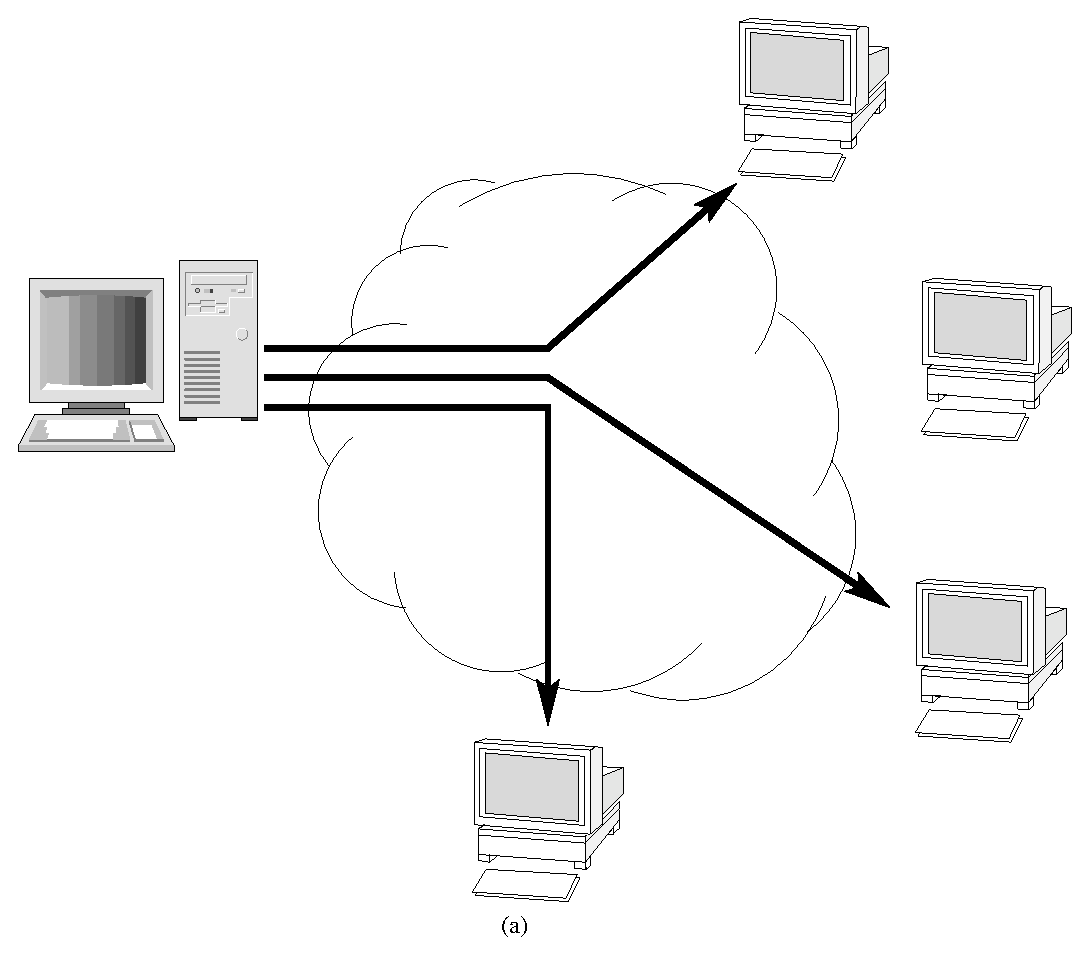
\includegraphics[width=2in]{figures/uniuni.eps}
\hspace{1in}
\includegraphics[width=2in]{figures/unimulti.eps}
\caption{(a) Unicasting the same data to multiple recipients; (b)
Doing the same thing with multicast.\label{unimulti}}
\end{center}
\end{figure}

Or consider a typical case where the sender has a single connection to
the Internet, such as a cable or DSL modem.  Sending the same data to
multiple recipients scattered throughout the Internet with unicast
requires that the same information be sent over that link many times
(\Fig{unimulti}a).  If the sender's first-hop connection has limited
outgoing capacity (say, one 1 Mbps or so), it may not even be
\emph{possible\/} to send some kinds of information---say, a real-time
video stream at 1 Mbps---to more than one recipient without exceeding
the first-hop link capacity, resulting in many lost packets and
poor quality.
%
Clearly it would be more efficient
if the information could be duplicated \emph{after\/} it crosses the first
link, as in \Fig{unimulti}b.
This saves bandwidth \emph{and\/} simplifies life for the sending program.

You may be surprised to learn that the sockets interface over TCP/IP
provides access to services like this---albeit with some
restrictions.  There are two types of
network duplication service: \defn{broadcast} and \defn{multicast}.
With broadcast, the program calls \fcnsys{sendto()}
once and the message is automatically delivered
to \emph{all\/} hosts on the local network.
With multicast, the message is sent once, and delivered
to a specific (possibly empty) \emph{group\/} of hosts throughout the
Internet---namely, those that have
indicated to the network that they should receive messages sent to that group.

\callout{We mentioned that there are some restrictions on these services.
The first is that \emph{only UDP sockets can use broadcast and
multicast services}.  The second is that \emph{broadcast only covers a local
scope}, typically a local area network.
The third restriction is that \emph{multicast across the entire
Internet is presently not supported by most Internet service
providers}.}
In spite of these restrictions, these services can often be useful.
For example, it is often useful to use multicast within a site such
as a campus network, or broadcast to local hosts.

\subsection{Broadcast}

\noindent UDP datagrams can be sent to all nodes on an attached local
network by sending them to a special address.  In IPv4 it is
called the ``limited broadcast address'', and it is the all-ones
address (in dotted-quad notation, 255.255.255.255).
In IPv6 it is called the ``all-nodes address (link scope)'', and has
the value % XXX formatting...
FF02::1.  Routers do not forward packets addressed to either one of
these addresses, so neither one will take a datagram beyond the local
network to which the sender is connected.  Each does,
however, deliver the sent packet to \emph{every\/} node on the
network; typically this is achieved using the hardware broadcast
capability of the local network. (Not all links support broadcast; in
particular, point-to-point links do not.  If
none of a host's interfaces support broadcast, any attempt to use it
will result in an error.)
Note also that a broadcast UDP datagram will actually be ``heard'' at a host
only if some program on that
host is listening for datagrams on the \emph{port\/} to which the
datagram is addressed.

What about a network-wide broadcast address to send a message to all
hosts?  There is no such address.  To see
why, consider the impact on the network of a broadcast to every host on
the Internet.  The send of a single datagram would result in a very, very
large
number of packet duplications by the routers, and bandwidth would be
consumed on each and every network.  The consequences of misuse
(malicious or accidental) are too great, so the designers of IP left
out such an Internet-wide broadcast facility  on purpose.   Even with these
restrictions, broadcast on the local link can be very useful.  Often it is
used in state exchange for network games where the players are all on
the same local area network (e.g., Ethernet).

There is one other difference between a broadcast sender and a regular
sender:  before sending to the broadcast address, the special socket
option \const{so\_broadcast} must be set.  In effect, this asks the
system for ``permission'' to broadcast.
%
We demonstrate the use of
UDP broadcast in \file{BroadcastSender.c}.  Our sender broadcasts 
a given string every three seconds to the limited broadcast address of
the address family indicated by the first argument.

\jcode{BroadcastSender.c}{code/BroadcastSender.c}{1}{1}

\begin{topcode}

\tlcitem{Declare constant address}{9}

Somewhat surprisingly, the all-nodes group address is not defined as a
named system constant, so we give it a name here.

\tlcitems{Parameter processing}{14--19}

\tlcitems{Destination address storage}{20--21}

We use a \type{sockaddr\_storage} structure to hold the destination
broadcast address, since it may be either IPv4 or IPv6.

\tlcitems{Setting up destination address}{24--47}

We set the destination address according to the given type, and
remember the size for later use.  Finally, we save the address in a
pointer to a generic type{sockaddr}.

\tlcitems{Socket creation}{53--56}

\tlcitems{Setting permission to broadcast}{59--63}
By default, sockets cannot broadcast.  Setting the
\const{SO\_BROADCAST} option
for the socket enables socket broadcast.

\tlcitem{Repeatedly broadcast}{65--72}
Send the argument string every three seconds to all hosts on the network.
\end{topcode}

Note that a receiver program does not need to do anything special to
receive broadcast datagrams (except bind to the appropriate port).
Writing a program to receive the broadcasts sent out by
\file{BroadcastSender.c} is left as an exercise.

\subsection{Multicast}

Using multicast is very similar to using unicast, for the sender.
The difference is in the form of the address.
A multicast address identifies a set of receivers who have ``asked''
the network to deliver messages sent to that address.  (This is the
receiver's responsibility; see below.)
A range of the address space is set aside for multicast in both IPv4
and IPv6.  IPv4 multicast addresses are in the range
224.0.0.0 to 239.255.255.255.  IPv6 multicast addresses are those
whose first byte contains 0xFF, i.e., all ones.  The IPv6 multicast
address space has a fairly complicated structure that is mostly beyond
the scope of this book. (The reader is referred to~\cite{RFC4291} for
details.)  For our examples we'll use
addresses beginning with FF1E; they are valid for transient use in global
applications.
(The third hex digit ``1'' indicates a multicast address that
is not permanently assigned for any particular purpose, while the
fourth digit ``E'' indicates global scope.)  An example would be FF1E::1234.

Our example multicast sender, shown in file
\file{MulticastSender.c}, takes a multicast address and
port as an argument, and sends a given string to that address and port
every three seconds.

\jcode{MulticastSender.c}{code/MulticastSender.c}{1}{1}

Note that unlike the broadcast sender, the
multicast sender does not need to set the
permission to multicast.  On the other hand, the multicast sender
may set the \emph{TTL\/} (``time-to-live'') value for the transmitted
datagrams.
Every packet contains a counter, which is initialized to
some default value when the packet is first sent,
and decremented by each router that handles the packet.  
When this counter reaches 0, the packet is discarded.  The TTL mechanism
(which can be changed by setting a socket option) allows us to
control the initial value of this counter, and thus
limit the number of hops a multicast packet can traverse.
For example, by setting TTL=1, the multicast packet  will not
go beyond the local network.

As mentioned above, the multicast network service duplicates and delivers
the message only to a specific set of receivers
This set of receivers, called a
\defn{multicast group}, is identified by a particular
multicast (or group) address.
These receivers need some mechanism to notify the network of
their interest in receiving data sent to a particular multicast
address.  Once notified, the network can begin forwarding the multicast
messages to the receiver.  This notification of the network,
called ``joining a
group,'' is accomplished via a multicast request (signaling)
message sent
 (transparently)
by the underlying protocol implementation.  To cause this to 
happen, the receiving program needs to invoke an
address-family-specific  multicast socket option.
For IPv4 it is  \const{ip\_add\_membership}; for IPv6 it is 
(surprisingly enough) \const{ipv6\_add\_membership}.
This socket option takes a structure containing the address of the
multicast ``group'' to be joined.  Alas, this structure is
also different for the
two versions:
\begin{inlinecode}
struct ip_mreq {
  struct in_addr imr_multiaddr; // Group address
  struct in_addr imr_interface; // local interface to join on
};
\end{inlinecode}
The IPv6 version differs only in the type of addresses it contains:
\begin{inlinecode}
struct ipv6_mreq {
  struct in6_addr ipv6mr_multiaddr; // IPv6 multicast address of group
  unsigned int ipv6mr_interface;    // local interface to join no
  };
\end{inlinecode}
Our multicast receiver contains
a fair amount of  version-specific code to handle the joining process.

\jcode{MulticastReceiver.c}{code/MulticastReceiver.c}{1}{1}

The multicast receiver joins the group, waits to receive a message,
prints it, then exits.

\subsection{Broadcast vs. Multicast}

The decision of using broadcast or multicast in an application
depends on several issues, including the fraction
of network hosts interested in
receiving the data, and the knowledge of the communicating parties.
Broadcast works well if a large percentage of the network hosts wish
to receive the message; however, if few hosts need to receive the
packet, broadcast ``imposes on'' all hosts in the network for the
benefit of a few.
Multicast is preferred, because it limits the duplication of data to
only those that have  expressed interest.
%
The disadvantages of multicast are (i) it is presently not supported globally,
and (ii) the sender and receiver must
agree on an IP multicast address in advance.
Knowledge of an address is not required
for broadcast.  In some contexts (local), this makes broadcast a better
mechanism for discovery than multicast.  All hosts can receive
broadcast by default, so it is simple to ask all hosts a question like
``Where's the printer?''  On the other hand, for wide-area applications,
multicast is the only choice.

\begin{exercises}

\item State precisely the conditions under which an iterative server
is preferable to a multiprocessing server.

\item Would you ever need to implement a timeout in a client or
  server that uses TCP?

\item Why do we make the server socket nonblocking in
\file{UDPEchoServer-SIGIO.c}?  In particular, what bad thing might
happen if we did not?


\item How can you determine the minimum and maximum allowable sizes for
  a socket's send and receive buffers?  Determine the minimums for
  your system.

\item \label{ex:sigpipe} This exercise considers the
reasoning behind the \constsys{sigpipe} mechanism a little further.
Recall that \constsys{sigpipe} is delivered when a program tries  to
send on a TCP socket whose connection has gone away in the meantime.
An alternative approach would be to simply have the \fcn{send()} fail
with \constsys{econnreset}.  Why might the signal-based approach be
better than conveying this information by return value?

\item What do you think will happen if you use the program in
  \file{MulticastReceiver.c} while the program
  \file{BroadcastSender.c} is running on a host connected to the same LAN?

\end{exercises}
